\documentclass[t,usenames,dvipsnames]{beamer}
\usetheme{Copenhagen}
\setbeamertemplate{headline}{} % remove toc from headers
\beamertemplatenavigationsymbolsempty

\usepackage{amsmath, tkz-euclide, tikz, xcolor, pgfplots, array}
\usetkzobj{all}
\pgfplotsset{compat = 1.16}
\usetikzlibrary{arrows.meta, calc, decorations.pathreplacing}
\pgfplotsset{every axis/.append style = {axis lines = middle, axis line style = {<->}}}
\pgfplotsset{every tick label/.append style={font=\tiny}}
\everymath{\displaystyle}

\title{Area of Triangles}
\author{}
\date{}

\AtBeginSection[]
{
  \begin{frame}
    \frametitle{Objectives}
    \tableofcontents[currentsection]
  \end{frame}
}

\begin{document}

\begin{frame}
    \maketitle
\end{frame}

\begin{frame}{Derivation of Area Formula}
\begin{minipage}{0.4\textwidth}
\raisebox{2cm}{
\begin{tikzpicture}
    \tkzDefPoints{0/0/A, 3/0/C, 2/1.5/B}
    \tkzDrawPolygon(A,B,C)
    \tkzLabelPoints[left](A)
    \tkzLabelPoints[above](B)
    \tkzLabelPoints[right](C)
    \tkzLabelSegment[below](A,C){$b$}
    \tkzLabelSegment[above](A,B){$c$}
    \tkzLabelSegment[above](B,C){$a$}
    \tkzDrawAltitude[color=red](A,C)(B)   \tkzGetPoint{D}
    \tkzMarkRightAngles[color=red](B,D,A C,D,B)
    \tkzLabelSegment[left, color=red](B,D){$h$}
\end{tikzpicture} }
\end{minipage}
\begin{minipage}{0.3\textwidth}
\begin{align*}
    \onslide<2->{\text{Area} &= \frac{1}{2}b{{\color{red}h}}  \\[8pt]}
    \onslide<3->{\sin A &= \frac{{\color{red}h}}{c} \\[8pt]}
    \onslide<4->{{\color{red}h} &= c\sin A   \\[8pt]}
    \onslide<5->{\text{Area} &= \frac{1}{2}bc\sin A \\}
\end{align*}
\end{minipage}
\end{frame}

\section{Find the area of a SAS triangle}

\begin{frame}{Find the Area of a SAS Triangle}
    The previous formula can be extended to find the area of a SAS triangle given any 2 side lengths and the angle measure between them:
    \[
    \text{Area} = \frac{1}{2}bc\sin A = \frac{1}{2}ac\sin B = \frac{1}{2}ab\sin C
    \]
\pause
In other words,
\[
\text{Area} = \frac{1}{2}\times \text{product of 2 sides} \times \text{sine of angle between them}
\]
\end{frame}

\begin{frame}{Example 1}
    Find the area of each triangle. Round your answers to 2 decimal places.   \newline\\
    
    $A = 62^\circ, b = 10, c = 24$ \newline\\
    \pause
    \begin{minipage}{0.45\textwidth}
    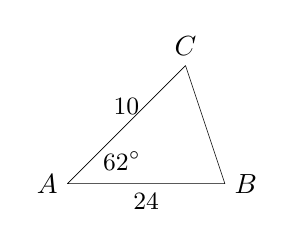
\begin{tikzpicture}
        \tkzDefPoints{0/0/A, 2/0/B, 1.5/1.5/C}
        \tkzDrawPolygon(A,B,C)
        \tkzLabelPoints[left](A)
        \tkzLabelPoints[right](B)
        \tkzLabelPoints[above](C)
        \tkzLabelAngle[pos=0.75](B,A,C){\small $62^\circ$}
        \tkzLabelSegment[above](A,C){\small 10}
        \tkzLabelSegment[below](A,B){\small 24}
    \end{tikzpicture}
    \end{minipage}
    \begin{minipage}{0.4\textwidth}
    \begin{align*}
        \onslide<3->{\text{Area} &= \frac{1}{2}(10)(24)\sin 62^\circ \\[12pt]}
        \onslide<4->{&\approx 105.95 \text{ sq. units}}
    \end{align*}
    \end{minipage}
\end{frame}

%%%%%%%%%%%%%%%%%%%%%%%%%%%%%%%%%%%%%%%%%%%%%%

\section{Find the area of an ASA or AAS triangle}

\begin{frame}{Needing Law of Sines}
    Sometimes, you must use the \alert{Law of Sines} to get enough information to find the area.   
    \[
    \frac{\sin A}{a} = \frac{\sin B}{b} = \frac{\sin C}{c}
    \]
\end{frame}

\begin{frame}{Example 2}
Find the area of each triangle. Round your answers to 2 decimal places. \newline\\
(a) \quad $a = 5, B = 149^\circ, C = 16^\circ$   \newline\\
\pause
\begin{tikzpicture}
\tkzDefPoints{0/0/A, 3/0/B, 2.25/1.5/C}
\tkzDrawPolygon(A,B,C)
\tkzLabelPoints[above](C)
\tkzLabelPoints[left](A)
\tkzLabelPoints[right](B)
\tkzLabelSegment[right](B,C){\small 5}
\tkzLabelAngle[pos=0.6](A,B,C){\small$149^\circ$}
\tkzLabelAngle[pos=0.5](B,C,A){\small$16^\circ$}
\end{tikzpicture}
\end{frame}

\begin{frame}{Example 2}
\begin{minipage}{0.4\textwidth}
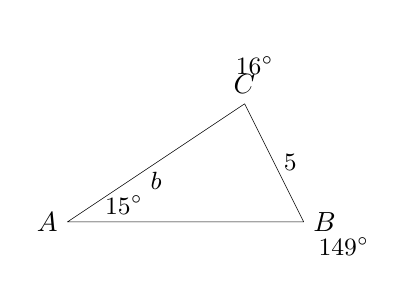
\begin{tikzpicture}
\tkzDefPoints{0/0/A, 3/0/B, 2.25/1.5/C}
\tkzDrawPolygon(A,B,C)
\tkzLabelPoints[above](C)
\tkzLabelPoints[left](A)
\tkzLabelPoints[right](B)
\tkzLabelSegment[right](B,C){\small 5}
\tkzLabelSegment[](A,C){\small $b$}
\tkzLabelAngle[pos=0.6](A,B,C){\small$149^\circ$}
\tkzLabelAngle[pos=0.5](B,C,A){\small$16^\circ$}
\tkzLabelAngle[pos=0.75](B,A,C){\small$15^\circ$}
\end{tikzpicture}
\end{minipage}
\hspace{0.25in}
\begin{minipage}{0.4\textwidth}
\begin{align*}
    \onslide<1->{\frac{\sin 15}{5} &= \frac{\sin 149}{b}} \\[10pt]
    \onslide<2->{b\sin 15 &= 5\sin 149}   \\[10pt]
    \onslide<3->{b &= \frac{5\sin 149}{\sin 15} \approx 9.95}    \\[10pt]
\end{align*}
\end{minipage}
\end{frame}

\begin{frame}{Example 2}
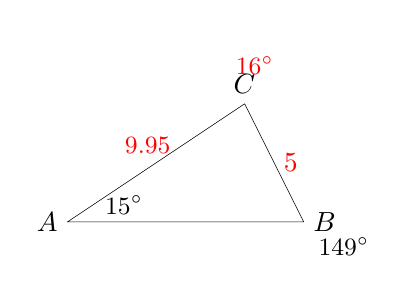
\begin{tikzpicture}
\tkzDefPoints{0/0/A, 3/0/B, 2.25/1.5/C}
\tkzDrawPolygon(A,B,C)
\tkzLabelPoints[above](C)
\tkzLabelPoints[left](A)
\tkzLabelPoints[right](B)
\tkzLabelSegment[right, color=red](B,C){5}
\tkzLabelSegment[color=red, above, xshift = -3pt](A,C){\small 9.95}
\tkzLabelAngle[pos=0.6](A,B,C){\small$149^\circ$}
\tkzLabelAngle[pos=0.5, color=red](B,C,A){\small$16^\circ$}
\tkzLabelAngle[pos=0.75](B,A,C){\small$15^\circ$}
\end{tikzpicture}
\newline\\
\pause
Area = $\frac{1}{2} \times 9.95 \times 5 \times \sin 16^\circ \approx \alert{6.86 \text{ sq. units}}$
\end{frame}

\begin{frame}{Example 2}
Find the area of each triangle. Round your answers to 2 decimal places. \newline\\
(b) \quad $c = 7, B = 132^\circ, A = 28^\circ$   \newline\\
\pause
\begin{tikzpicture}
\tkzDefPoints{0/0/A, 3/0/B, 2.25/1.5/C}
\tkzDrawPolygon(A,B,C)
\tkzLabelPoints[above](C)
\tkzLabelPoints[left](A)
\tkzLabelPoints[right](B)
\tkzLabelSegment[below](B,A){7}
\tkzLabelAngle[pos=0.6](A,B,C){\small$132^\circ$}
\tkzLabelAngle[pos=0.75](B,A,C){\small$28^\circ$}
\end{tikzpicture}
\end{frame}

\begin{frame}{Example 2}
\begin{minipage}{0.4\textwidth}
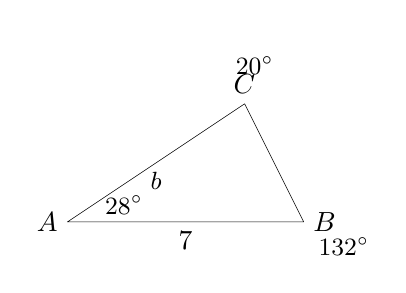
\begin{tikzpicture}
\tkzDefPoints{0/0/A, 3/0/B, 2.25/1.5/C}
\tkzDrawPolygon(A,B,C)
\tkzLabelPoints[above](C)
\tkzLabelPoints[left](A)
\tkzLabelPoints[right](B)
\tkzLabelSegment(A,C){\small $b$}
\tkzLabelSegment[below](B,A){7}
\tkzLabelAngle[pos=0.6](A,B,C){\small$132^\circ$}
\tkzLabelAngle[pos=0.75](B,A,C){\small$28^\circ$}
\tkzLabelAngle[pos=0.5](B,C,A){\small$20^\circ$}
\end{tikzpicture}
\end{minipage}
\hspace{0.25in}
\begin{minipage}{0.4\textwidth}
\begin{align*}
    \onslide<1->{\frac{\sin 20}{7} &= \frac{\sin 132}{b}} \\[10pt]
    \onslide<2->{b\sin 20 &= 7\sin 132}   \\[10pt]
    \onslide<3->{b &= \frac{7\sin 132}{\sin 20} \approx 15.21}    \\[10pt]
\end{align*}
\end{minipage}
\end{frame}

\begin{frame}{Example 2}
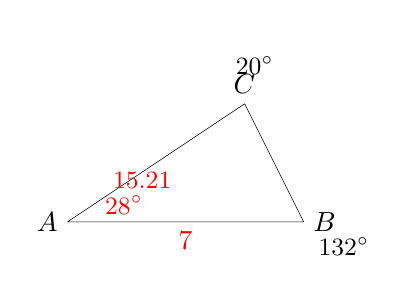
\begin{tikzpicture}
\tkzDefPoints{0/0/A, 3/0/B, 2.25/1.5/C}
\tkzDrawPolygon(A,B,C)
\tkzLabelPoints[above](C)
\tkzLabelPoints[left](A)
\tkzLabelPoints[right](B)
\tkzLabelSegment[color=red, below](B,A){7}
\tkzLabelSegment[xshift=-5pt, color=red](A,C){\small 15.21}
\tkzLabelAngle[pos=0.6](A,B,C){\small$132^\circ$}
\tkzLabelAngle[pos=0.75, color=red](B,A,C){\small$28^\circ$}
\tkzLabelAngle[pos=0.5](B,C,A){\small$20^\circ$}
\end{tikzpicture}
\newline\\
\pause
Area = $\frac{1}{2} \times 15.21 \times 7 \times \sin 28^\circ \approx \alert{24.99 \text{ sq. units}}$
\end{frame}

%%%%%%%%%%%%%%%%%%%%%%%%%%%%%%%%%%%%%%%%%%%%%%%%%%%%%%%%%%%%%%%%%

\section{Find the area of a SSS triangle}

\begin{frame}{Find the Area of a SSS Triangle}
While it is OK to use the area formulas that we have been using (after using Law of Cosines to find an angle measure) there is a quicker way to find the area of a SSS triangle by using \alert{Heron's Formula}.
\end{frame}

\begin{frame}{Heron's Formula}
    Let $s$ be the semi-perimeter of $\triangle ABC$:
    \[
    s = \frac{1}{2}(a+b+c)
    \]
Then
\[
\text{Area} = \sqrt{s(s-a)(s-b)(s-c)}
\]
\end{frame}

\begin{frame}{Example 3}
    Find the area of each triangle. Round your answers to 2 decimal places.    \newline\\
    
(a) \quad $a=11, b=13, c=12$    
\pause
\begin{align*}
    \onslide<2->{s &= \frac{1}{2}(11+13+12) = 18} \\[10pt]
    \onslide<3->{\text{Area} &= \sqrt{18(18-11)(18-13)(18-12)}}  \\[10pt]
    \onslide<4->{&\approx 61.48 \text{ sq. units}}
\end{align*}
\end{frame}

\begin{frame}{Example 3}
    Find the area of each triangle. Round your answers to 2 decimal places.    \newline\\
    
(b) \quad $a=8, b=10, c=15$    
\pause
\begin{align*}
    \onslide<2->{s &= \frac{1}{2}(8+10+15) = 16.5} \\[10pt]
    \onslide<3->{\text{Area} &= \sqrt{16.5(16.5-8)(16.5-10)(16.5-15)}}  \\[10pt]
    \onslide<4->{&\approx 36.98 \text{ sq. units}}
\end{align*}
\end{frame}

\end{document}
